\documentclass[12pt,parskip=half-]{scrartcl}
\usepackage{graphicx}
\usepackage[sorting=none,backend=biber,style=numeric]{biblatex}
\usepackage{float} % Change figure placement
\usepackage{hyperref} % Make urls, citations, and references clickable

% Make links blue and underlined
\hypersetup{
    colorlinks=true,
    citecolor=blue,
    linkcolor=blue,
    urlcolor=blue
}

\addbibresource{tex/references.bib}

% From float package: Always place figures in the right location
\floatplacement{figure}{H}

\title{COSC3000: Data visualisation report}
\author{John Owen\\Student ID: 43591617}
\date{}

\begin{document}

\maketitle

\section{Project aim}

The project uses data visualisation techniques to analyse two datasets, the
UCDP/PRIO Armed Conflict dataset, and the International Crisis Behavior Project
dataset. The aim is to gain insights into how wars change over time, the main
players involved, and the associations of nuclear weapon capability in
conflicts.

\section{Motivation}

The ever growing need to stop war before it starts and minimise loss of life
once it has does not need to be stated. Understanding war is key not only to
governments and institutions with the power to control it but also to the
citizens who must elect the government officials and political parties
that deal with its complexities.

War is usually understood through long texts that describe in detail all
recorded events. While this can give a thorough understanding of a particular
conflict, exploring war through statistics and graphs has many advantages.
Namely,

\begin{itemize}
    \item Wars can be understood at the macro level, looking at trends across
        many wars at once.
    \item Graphics can quickly give a rich summary difficult to describe in
        words.
    \item Wars can be distilled to one or two factors that the reader is
        interested in, allowing a quick comparison of these factors across many
        wars.
\end{itemize}

\section{Datasets used}

A combination of three publicly available data sources were used in the
project.

\subsection{UCDP/PRIO armed conflict dataset}

Contains a list of 259 conflicts ranging from 1946 to 2014
\cite{ucdpconflictsdataset, ucdpconflictscodebook, ucdpconflicts}. For each
conflict it lists:

\begin{itemize}
    \item Start and end date.
    \item Location.
    \item All states and non-state groups (henceforth collectively referred to
        as actors) on both sides of the conflict.
    \item Type of conflict (civil war, international war, other possibilities)
    \item Rough estimate of death count.
\end{itemize}

\subsection{Gleditch and Ward list of states}

Entries in the UCDP/PRIO dataset use numeric IDs to identify countries. This
dataset maps those IDs to the full names and three letter country codes of
states. For example, ``United States of America'' has an ID of 2 and a country
code of ``USA''. \cite{gwstatesdataset}

\subsection{International Crisis Behavior Project datasets}

Describes many dimensions of 470 international crises from 1918 to 2014.
Interestingly, rather than containing conflicts, it contains military security
crises, which the codebook defines as the period following a sudden increase in
the presence or threat of violence. This definition will be used in the rest of
the report. \cite{icbdataset, icbcodebook, icb}

The data comes in two datasets which in total have over 160 columns in total,
so it is too large to describe here. However, some example information it
contains for each crisis:

\begin{itemize}
    \item What was the cause of the crisis.
    \item Level of communication between crisis actors.
    \item Date and location of crisis.
    \item Crisis management style of crisis actors (e.g, negotiation,
        economic pressure, violence, etc).
    \item The role of any states involved in the crisis.
    \item The role of any global organizations (e.g, branches of the UN).
    \item Nuclear weapon capability of crisis actors.
\end{itemize}

\section{Method}

CSV files and tab separated value (TSV) files were obtained from publicly
viewable websites \cite{ucdpconflictsdataset, gwstatesdataset, icbdataset}. In
the case of the Gleditcsh and Ward list of states, two TSV files were combined
into one CSV file for easier data loading.  These datasets are located in the
\texttt{datasets/} directory.

The R language \cite{r} was used primarily in conjunction with its ``ggplot2''
\cite{ggplot2}, ``network'' \cite{networkmanual, networkarticle}, and
``GGally'' \cite{ggally} libraries to generate all graphs. The R code is
available in the \texttt{code/main.R} script file. The script loads the datasets,
converts columns to the correct data type (e.g, ``1'' is parsed as a number and
``1,2,3'' is parsed as a vector of numbers), and outputs diagrams.  For the
network diagrams, the data had to be carefully converted to an adjacency matrix
and pruned of boring data (e.g, nodes with no edges).

To build the project, see the \texttt{readme.md} file.

\section{Results}

\begin{minipage}{\textwidth}
    For all levels of violence, the frequency of crises peaked in the late 70's
    and drastically dropped afterwards (Fig \ref{war_over_time.pdf}). There are
    many possible reasons for this, but the most obvious candidate is the
    decline of the Cold War and the collapse of the Soviet Union.

    \begin{figure}
        \centering
        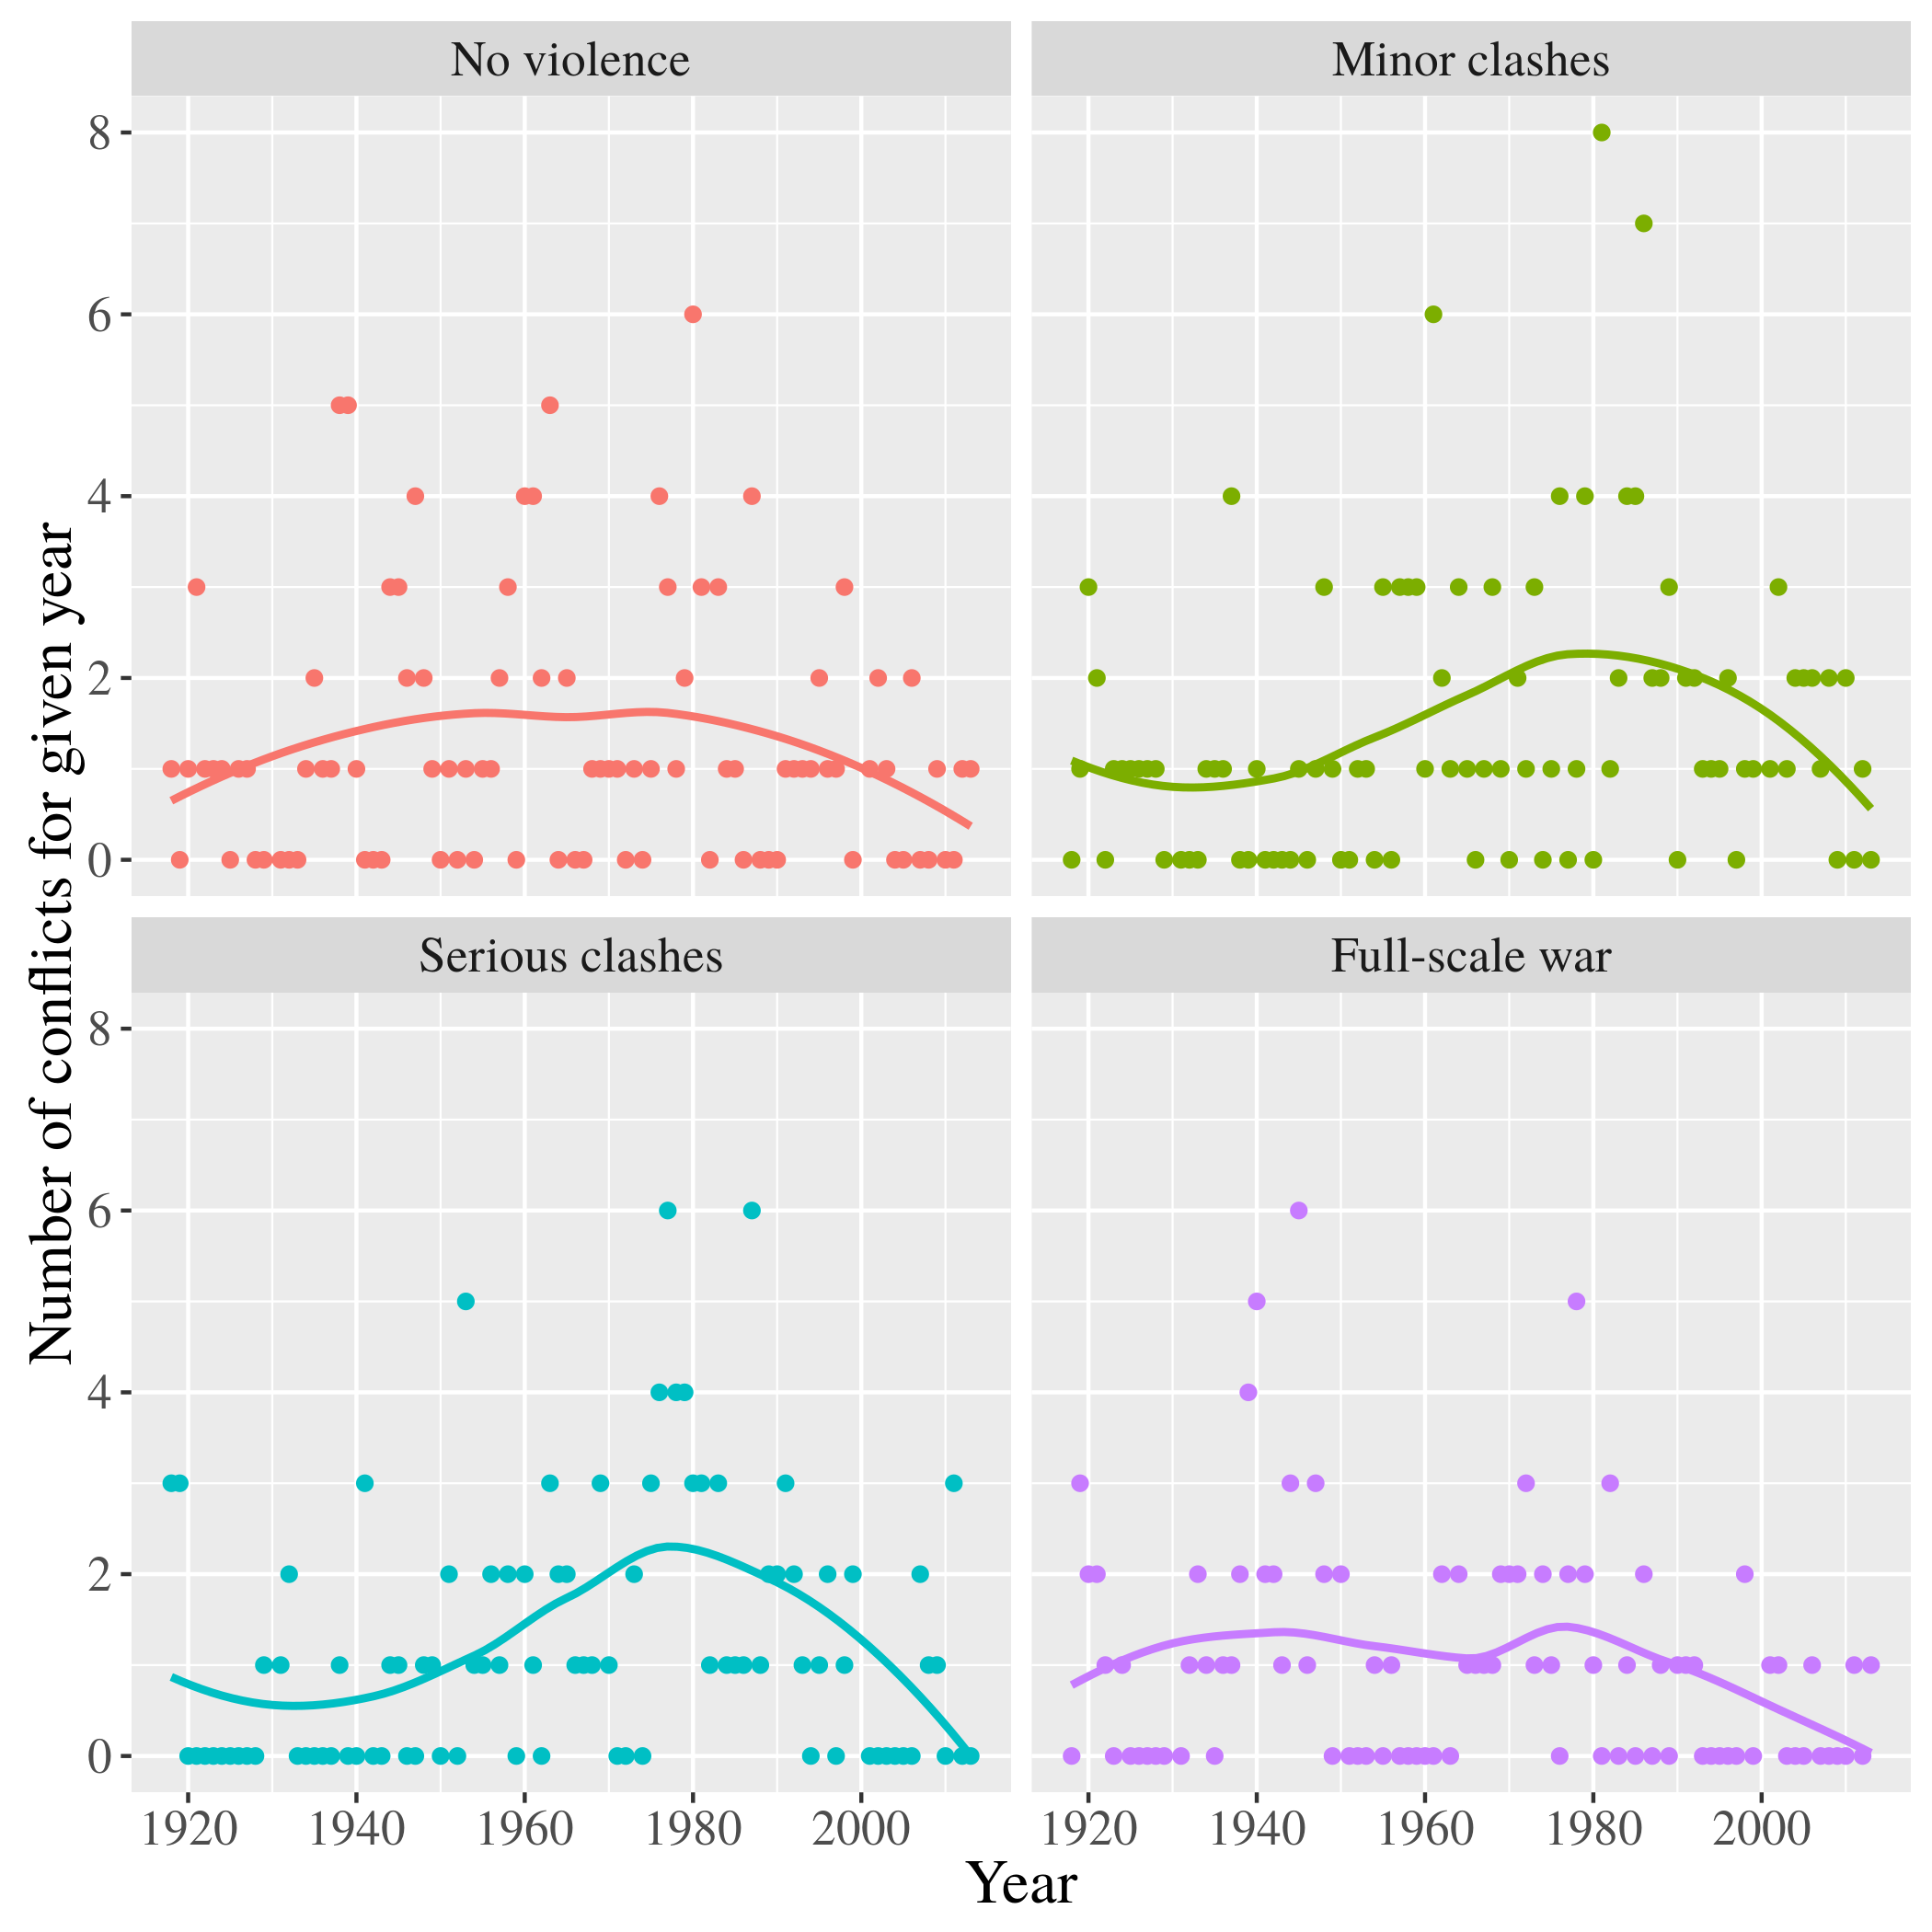
\includegraphics[width=\textwidth]{tmp/war_over_time.pdf}
        \caption{Violence in crises over time. Each dot represents the
            frequency of crises for a particular year. A Loess curve is fitted
        to the data to show the overall trend.}
        \label{war_over_time.pdf}
    \end{figure}
\end{minipage}

\begin{minipage}{\textwidth}
    An increase in the nuclear capabilities (see Appendix
    \ref{nuclearcapabilitydefs} for precise definitions of the levels of
    nuclear capabilities) of actors in a crisis is associated with a large
    increase in the frequency of non-violent crises vs frequency of violent
    crises (Fig \ref{nuclear_compared_with_violence.pdf}). However, there is a
    negligible difference between the frequency of non-violent crises where
    actors have the third level of nuclear capability (possession of nuclear
    weapons) vs the fourth level (second strike capability).

    \begin{figure}
        \centering
        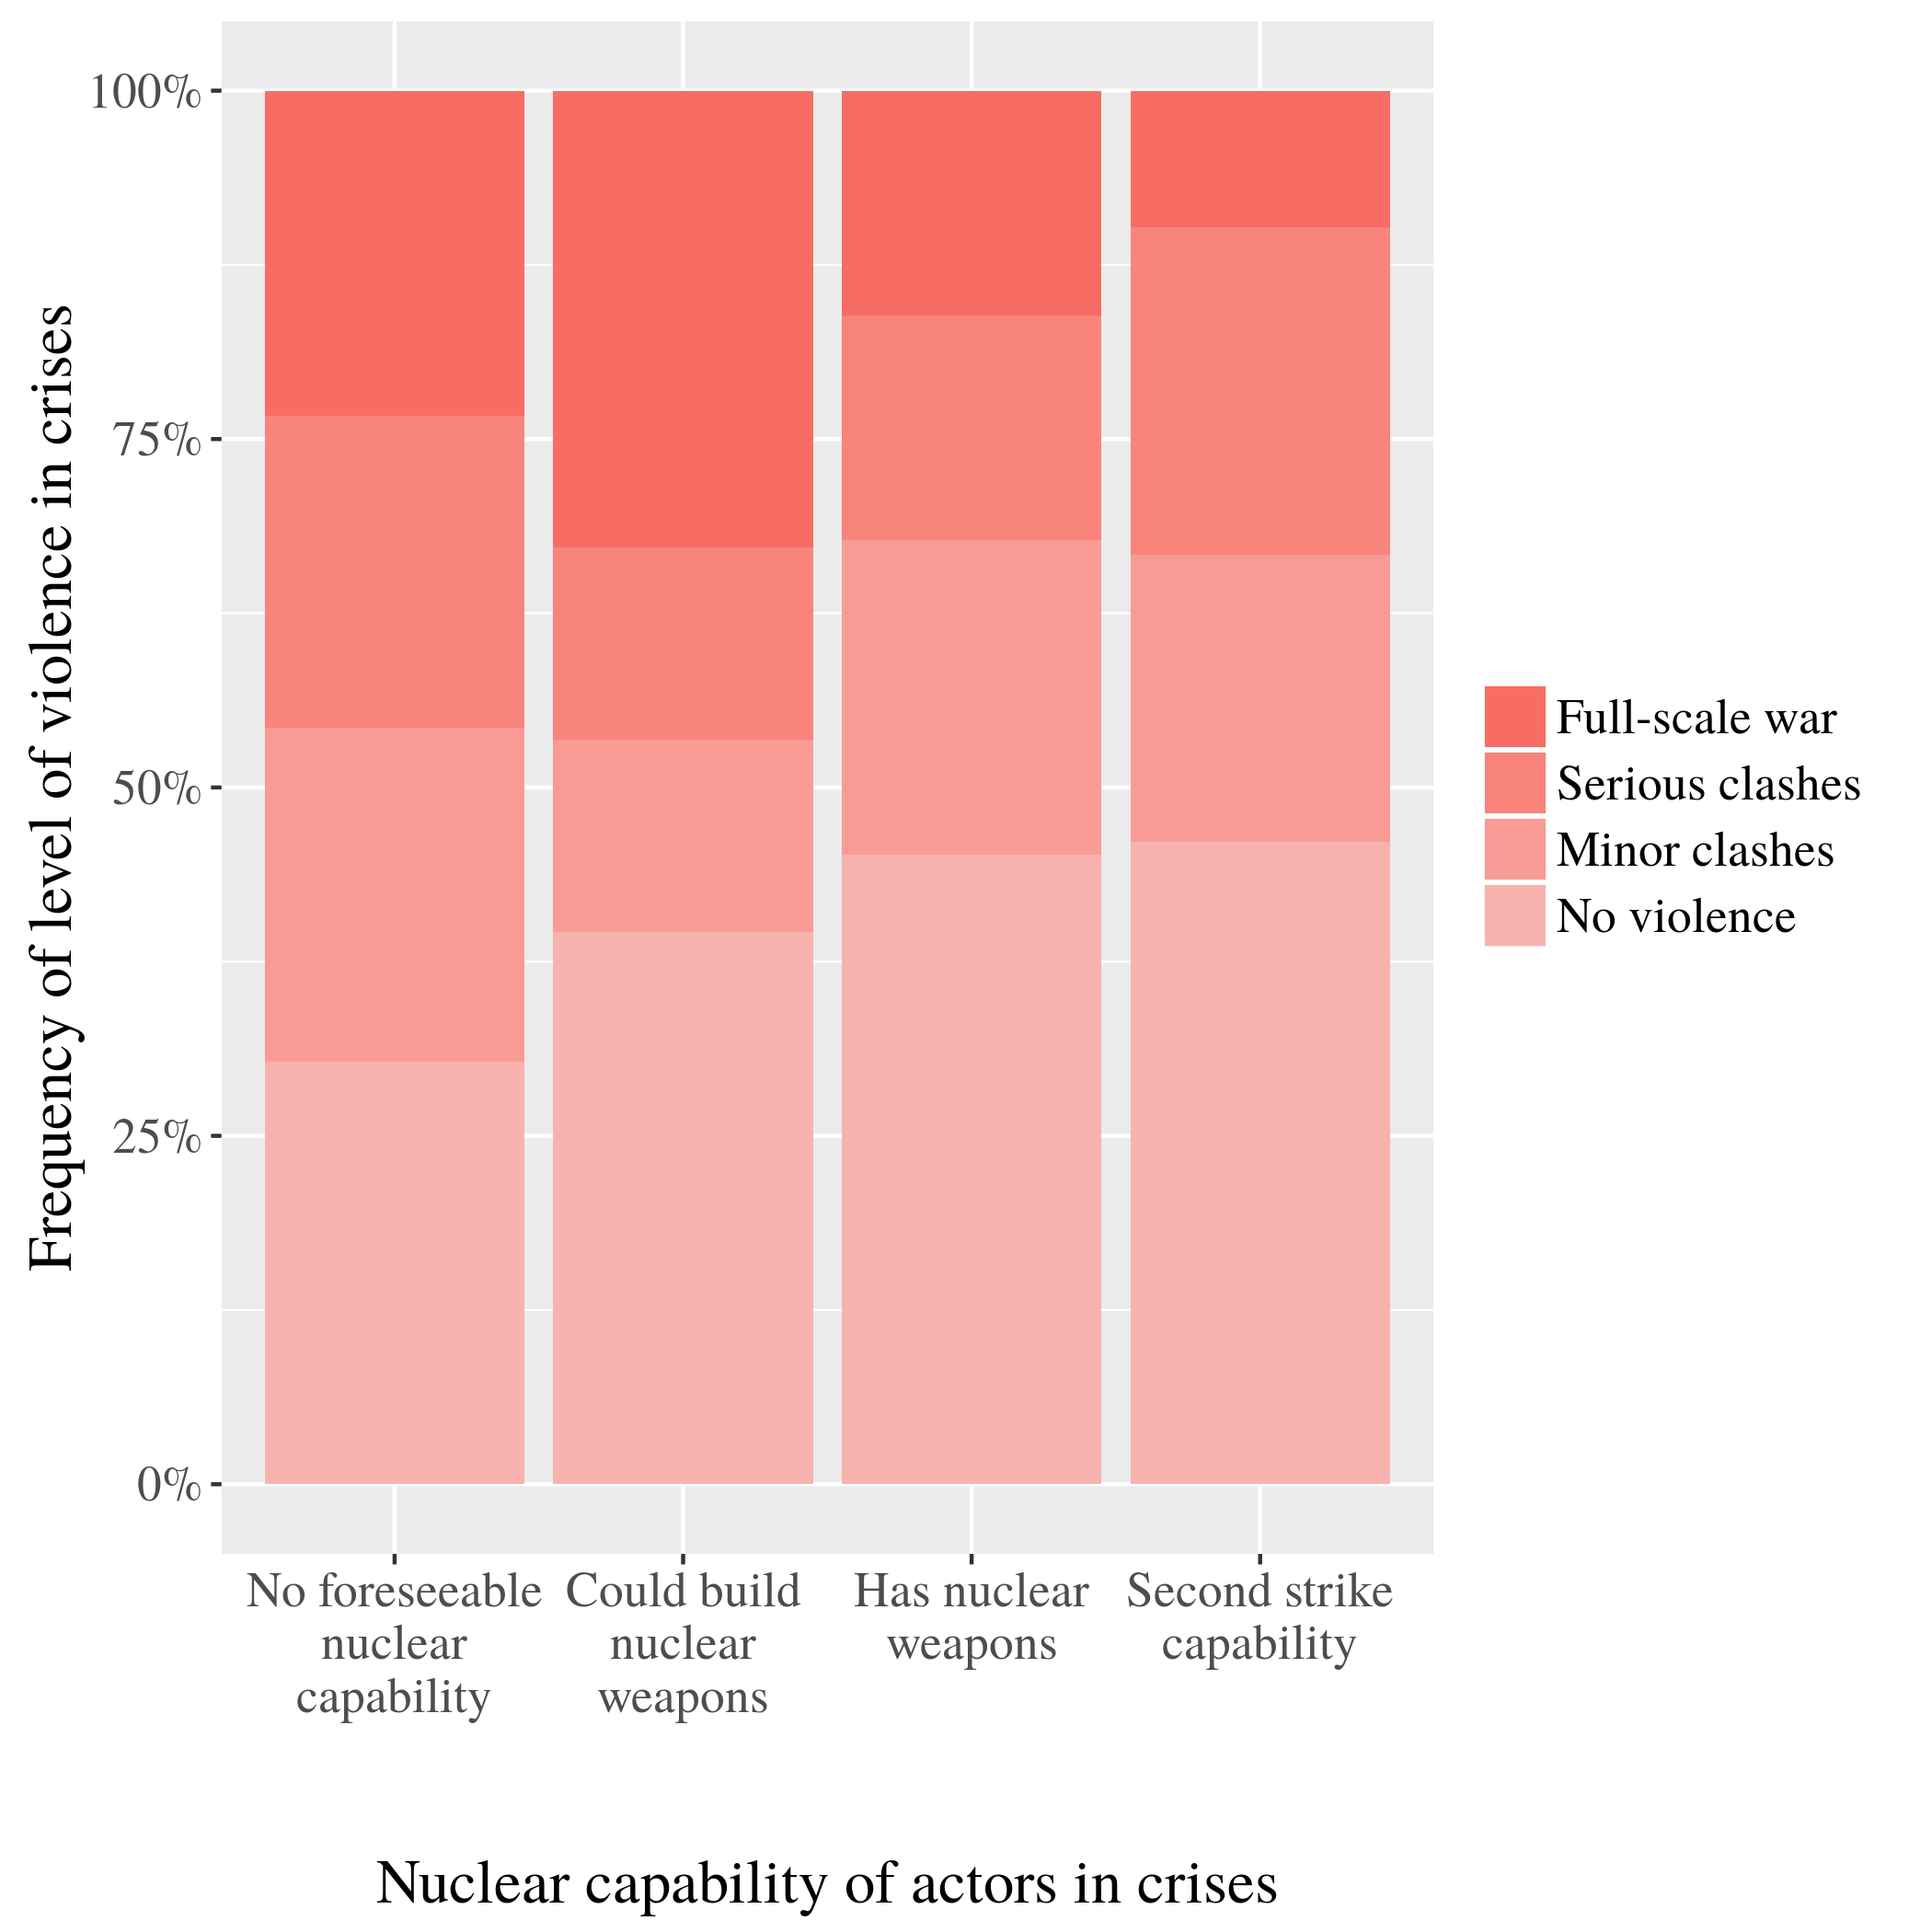
\includegraphics[width=0.75\textwidth]{tmp/nuclear_compared_with_violence.pdf}
        \caption{Country nuclear capability compared with crisis violence. See
            Appendix \ref{nuclearcapabilitydefs} for precise definitions of the nuclear
            capability levels.}
        \label{nuclear_compared_with_violence.pdf}
    \end{figure}

    The possession of nuclear weapons can decrease violent conflicts because
    states will avoid direct conflict to avoid triggering a mutually
    destructive nuclear war, as seen in the Cold War \cite{mad}. However, a
    hypothesis shared by some is that beyond a certain level of nuclear
    capability, further bolstering a nuclear arsenal doesn't lead to a decrease
    in conflict \cite{nukesvideo}. While this graph shouldn't be taken as
    evidence of that claim, this is the result that would be expected if it
    were true.
\end{minipage}

\begin{minipage}{\textwidth}
    Most countries that have fought wars, do so with only a small number of
    allies, generally one or two. A small number
    of countries (Malia, USA, Afghanistan, Iraq) have fought in wars with many
    allies. (Fig \ref{ally_network.pdf})

    \begin{figure}
        \centering
        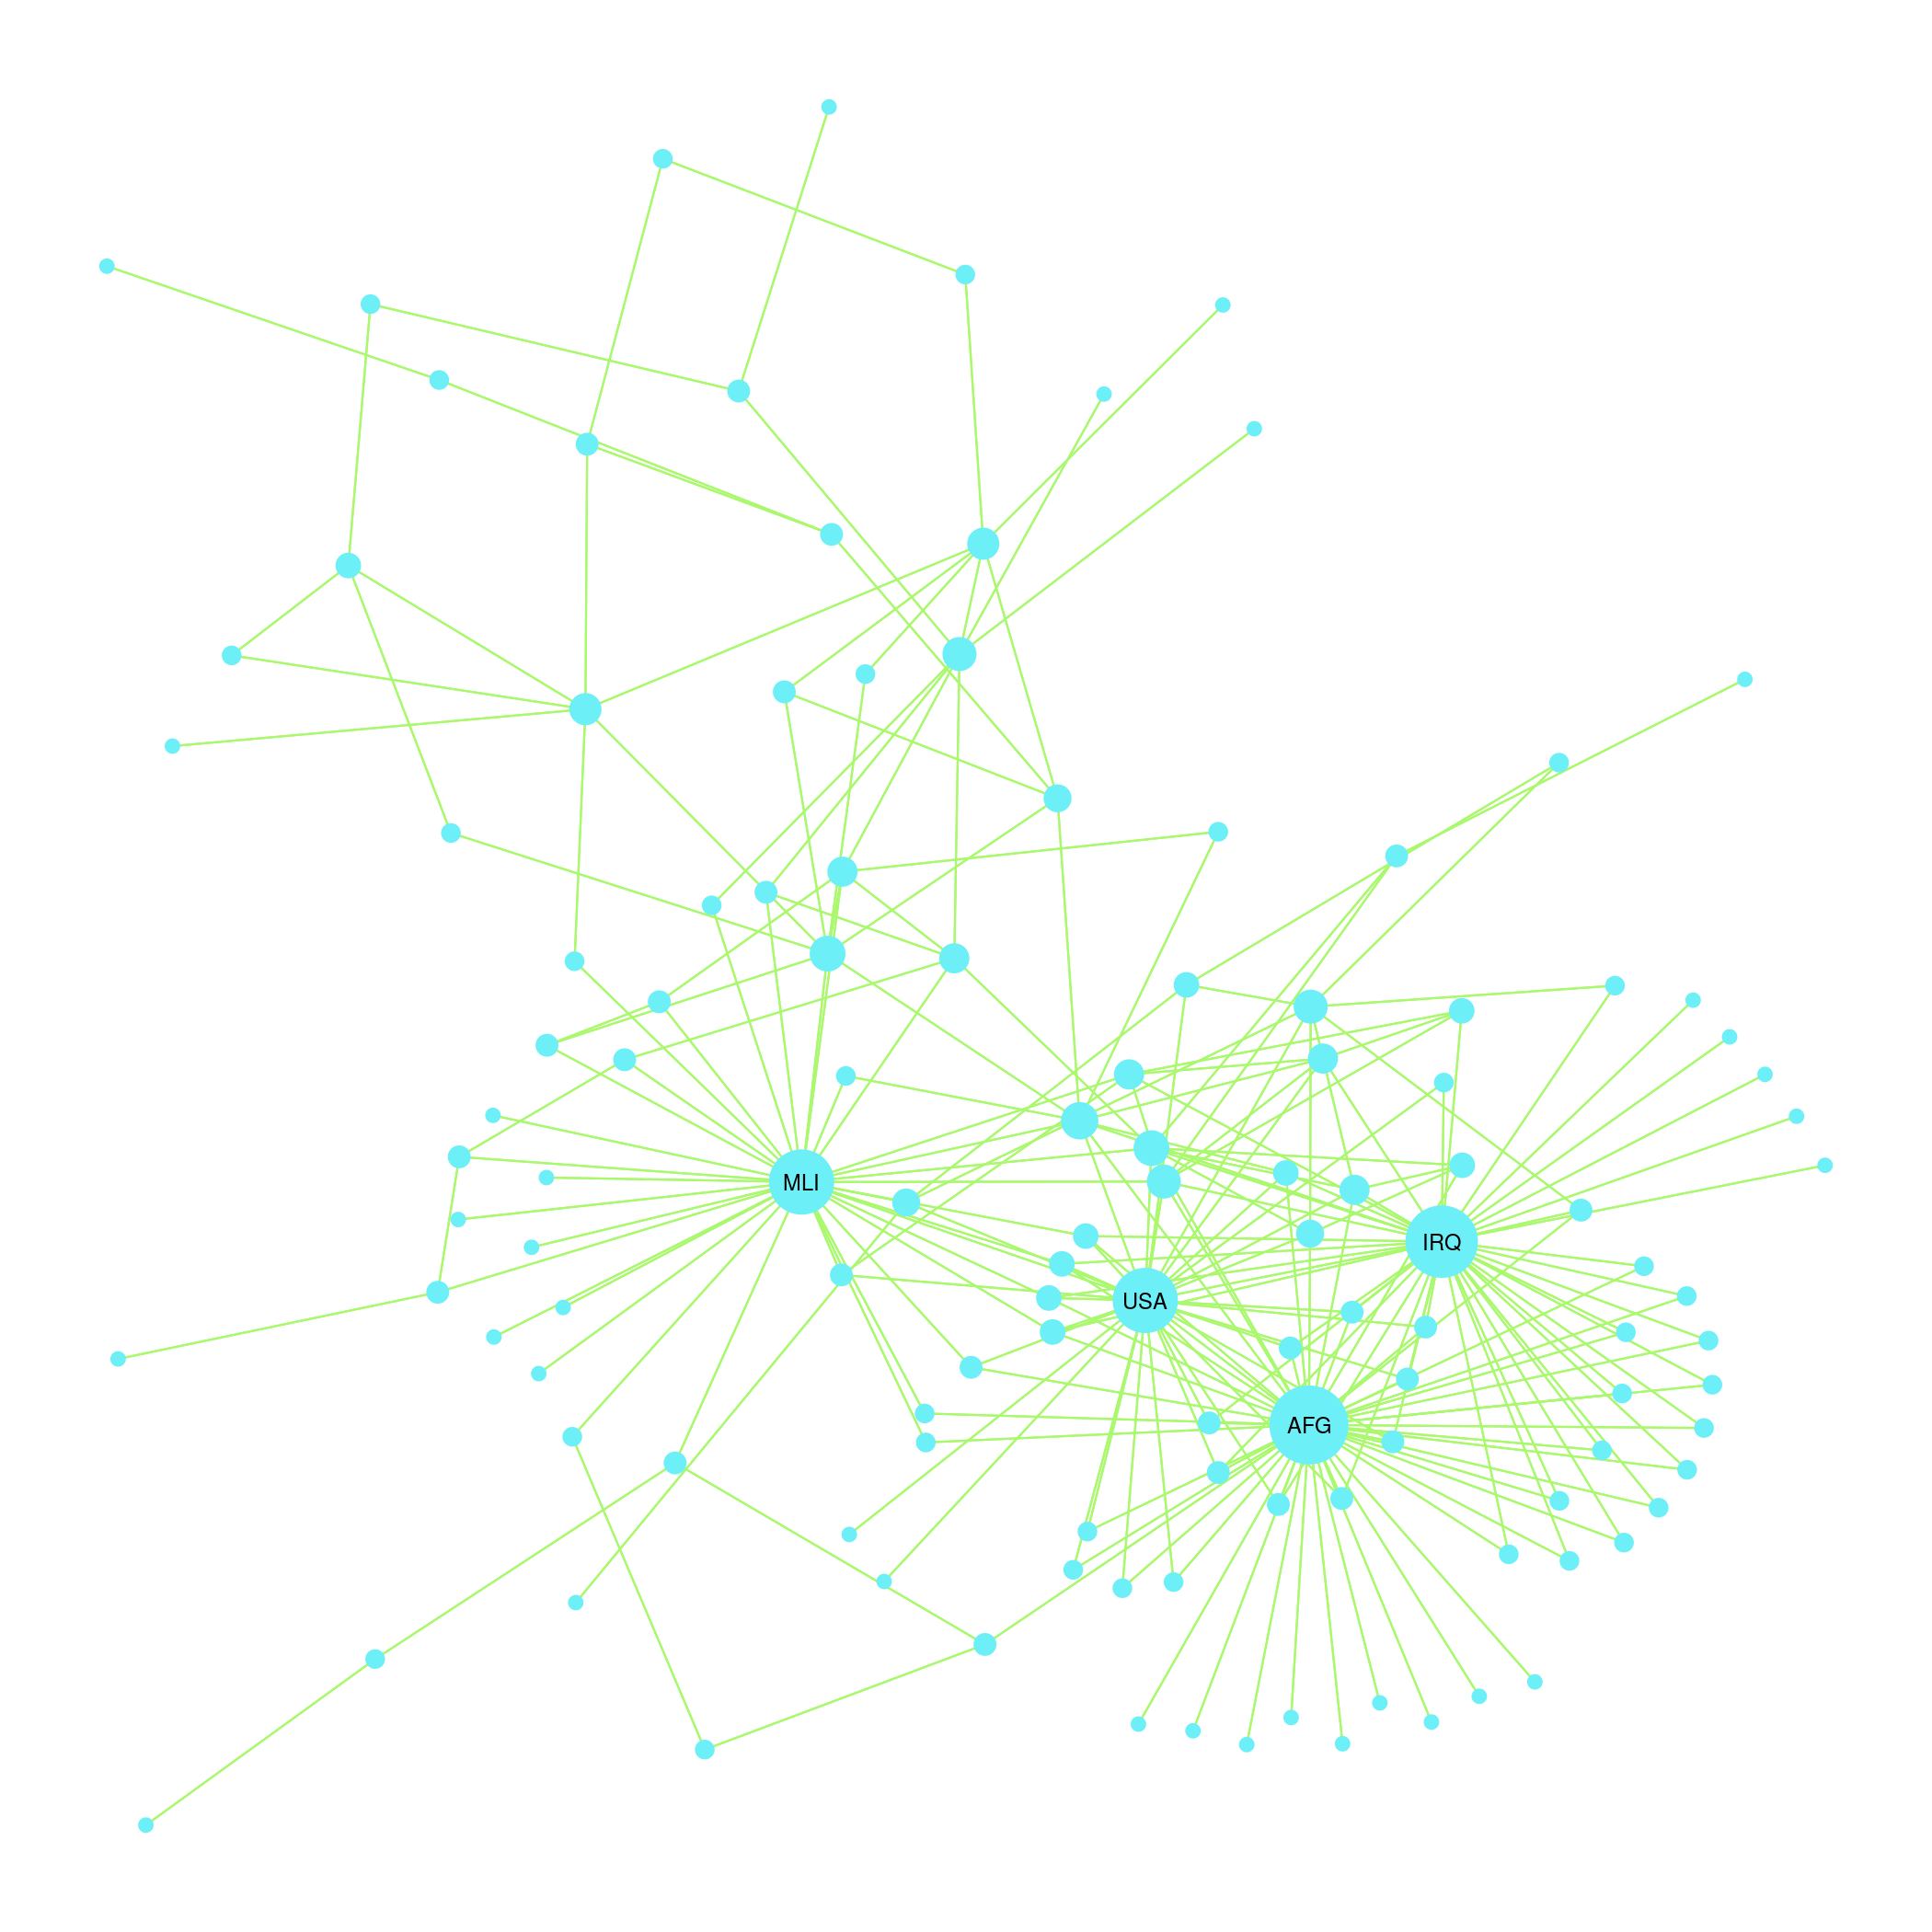
\includegraphics[width=\textwidth]{tmp/ally_network.pdf}
        \caption{A network plot of countries that have fought as allies. Each
            node is a country and every edge represents an instance where two
            countries have fought on the same side. Countries that have not had
            any allies in conflicts they have fought (i.e, nodes with no edges)
            are not displayed. Four countries which have fought with a far
            greater number allies have been labeled. These countries are Mali
            (MLI), The United States of America (USA), Afghanistan (AFG), and
            Iraq (IRQ). The size of each node is determined by the number of
            edges it has.}
        \label{ally_network.pdf}
    \end{figure}
\end{minipage}

\begin{minipage}{\textwidth}
    Most countries that have fought wars, have done so with a few opponents.  A
    few countries (Iraq, North Korea, Russia, China) have directly fought wars
    with many opponents (Fig \ref{enemy_network.pdf}).

    \begin{figure}
        \centering
        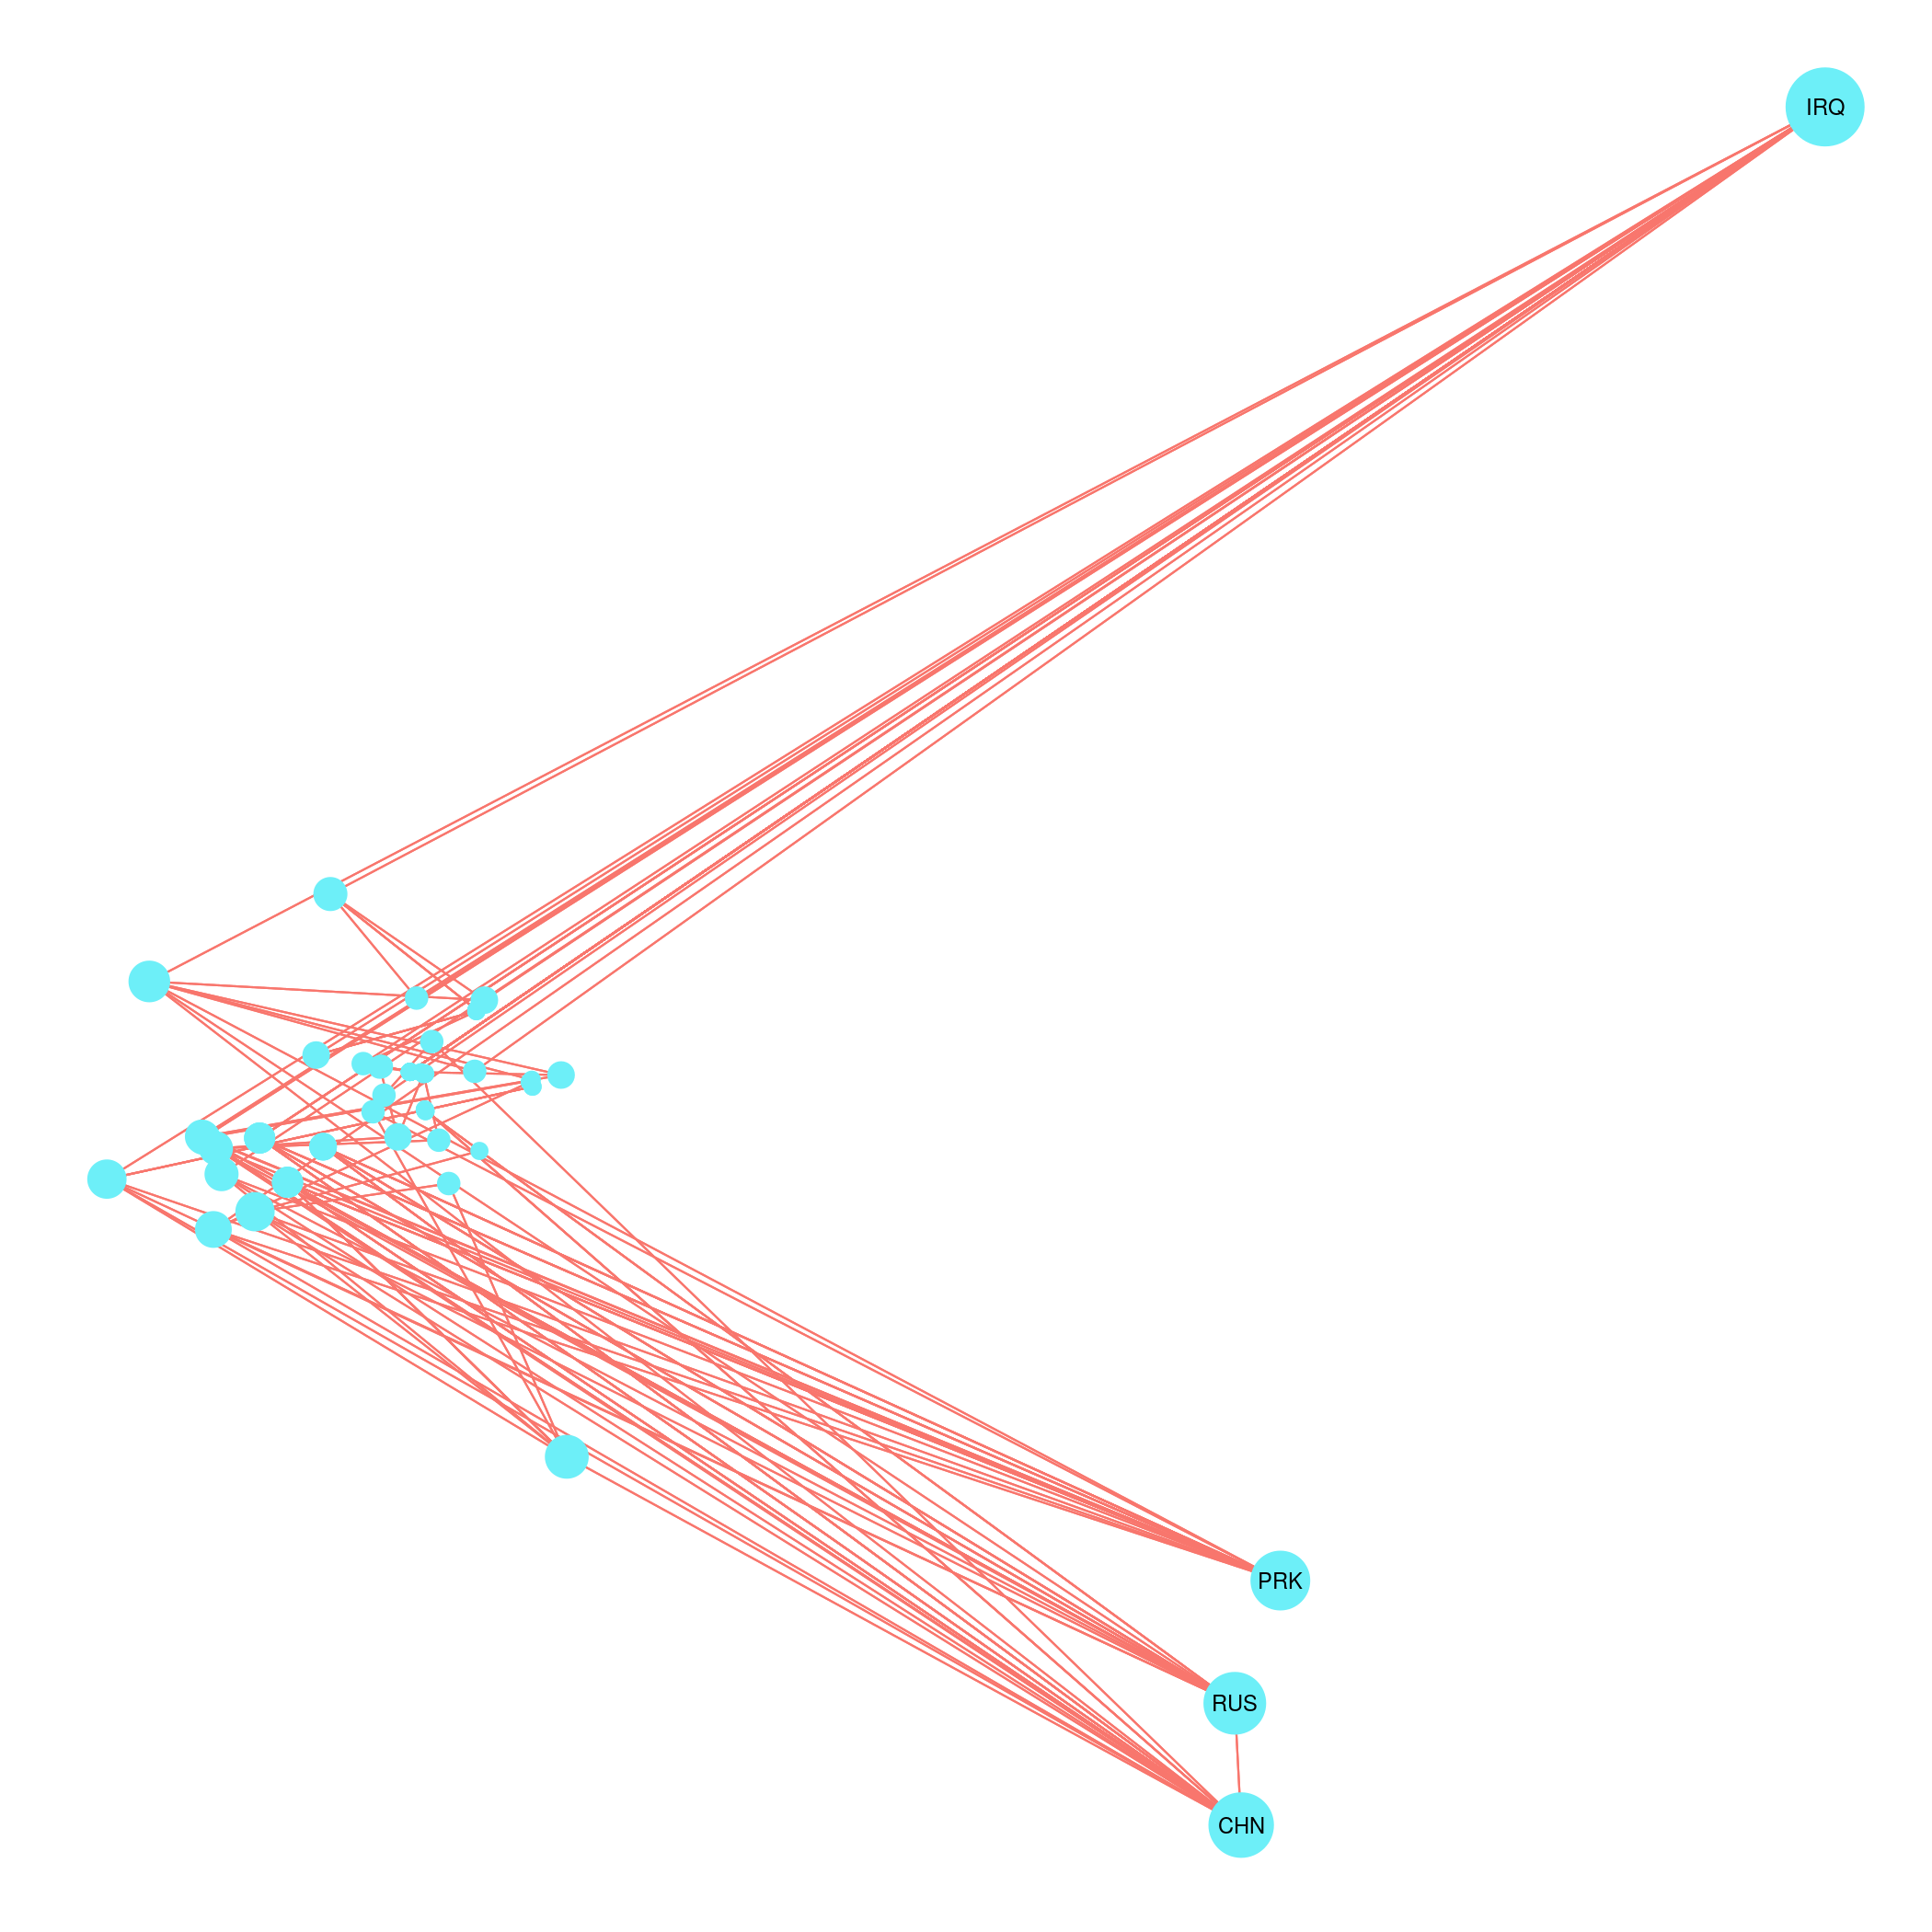
\includegraphics[width=\textwidth]{tmp/enemy_network.pdf}
        \caption{A network plot of countries that have fought as enemies. Each node
            is a country and every edge represents an instance where two countries
            have fought on opposing sides. Countries that have not been involved in
            any conflicts (i.e, nodes with no edges) are not displayed. Four
            countries which have fought with a far greater number of enemies have
            been labeled. These countries are Iraq (IRQ), North Korea (PRK),
            Russia (RUS), and China (CHN). The size of each node is determined
            by the number of edges it has.}
        \label{enemy_network.pdf}
    \end{figure}

    Interestingly, despite the USA's military power and its involvement in many
    theatres of conflict, it doesn't appear on the list of top countries. This
    is because after World War II, due to fears that a direct conflict with the
    Soviet Union could lead to a nuclear apocalypse, the USA engaged less often
    in combat and more often participated indirectly in proxy wars; often
    choosing to equip and train governments and rebel groups instead.
    \cite{mad}. 
\end{minipage}

\section{Appendix}
\appendix

\section{Nuclear capability levels}\label{nuclearcapabilitydefs}

Taken directly from the ICB dataset codebook \cite{icbcodebook}.

\begin{description}
    \item[No (foreseeable) nuclear capability] The actor did not possess a
        nuclear capability with any operational military significance when the
        crisis began; moreover, the international consensus at the time was
        that it could not develop or acquire such capability within five years.
    \item[Foreseeable nuclear capability] The actor could develop or acquire
        operational nuclear military capability within five years of the
        beginning of the crisis.
    \item[Possession of nuclear capability] the actor had nuclear military
        capability (weapons) and delivery means but no second-strike
        capability.
    \item[Developed nuclear capability, with second strike capability]
        Superpower or great power with ability to absorb a first strike and
        retaliate.
\end{description}

\nocite{*}
\printbibliography

\end{document}
